\chapter{Struktura Aplikacji}

Struktura aplikacji została częściowo opisana w rozdziale \hyperref[ch:manual]{\textbf{Podręcznik użytkownika}}.

\section{Edytor notatki}

Edytor notatki składa się z edytora tytułu znajdującego się w głównym pasku strony edycji notatki, oraz edytora zawartości.

\subsection{Zarządzanie zawartością}

Do zarządzania zawartością notatki używana jest klasa \textbf{NoteParagraphs} przechowująca listę obiektów typu \textbf{NoteParagraph} reprezentujących paragrafy notatki.
Współpracę tych klas można przedstawić w uproszczony sposób za pomocą schematu:

\begin{figure}[ht]
    \centering
    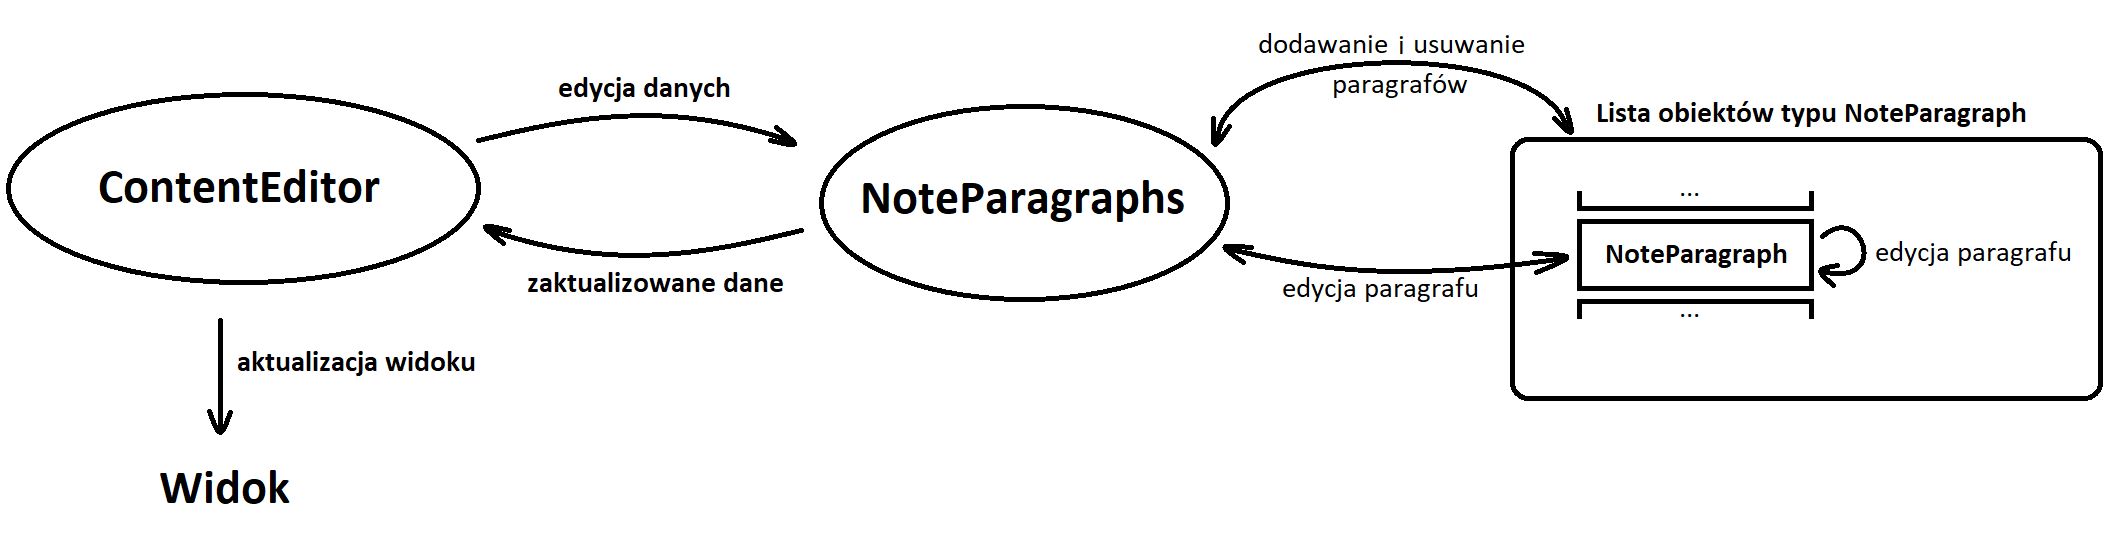
\includegraphics[width=\linewidth]{images/ContentEditor_podzial.png}
    \caption{Uproszczony schemat zarządzania paragrafami.}
\end{figure}

\subsection{Paragrafy}

Istanieją trzy typy paragrafów w edytorze dziedziczące po \textbf{NoteParagraph}: 
\begin{itemize}
    \item \textbf{NoteParagraphTextEditor},
    \item \textbf{NoteParagraphWidget},
    \item \textbf{NoteParagraphPlaceholder}
\end{itemize}

Każdy z paragrafów posiada unikalny identyfikator \textbf{id} oraz referencję do fabryki widgetów tworzonej wewnątrz managera \textbf{NoteParagraphs}.
Pozwala to na unikalne identyfikowanie paragrafów wewnątrz listy, oraz wszystkich utworzonych widgetów w obrębie przestrzenii edytora.

Używane są również mechanizmy wywołań zwrotnych(callbacks) do zgłaszania aktywności(focus) oraz zaistniałej zmiany, jak również usunięcia z listy na podstawie swojego id, gdy wszystkie jego elementy zostaną usunięte.

\subsubsection{NoteParagraphTextEditor}

Służy do przechowywania, wyświetlania i edycji tekstu notatki. Posiada mechanizmy dynamicznej zmiany rozmiaru poprzez manipulację stanem oraz wartościami wewnętrznych pól. Posiada tylko jeden element, którym jest pole tekstowe z niestandardowym kontrolerem używającym parsera tekstu.

\subsubsection{NoteParagraphWidget}

Służy do przechowywania, wyświetlania i edycji widgetów notatki. Posiada mechanizmy dynamicznej zmiany rozmiaru wraz ze zmianą rozmiaru widgetu będącego elementem głównym. Mechanizmy zmiany rozmiaru są różne w zależności od rodzaju widgetu.

\subsubsection{NoteParagraphPlaceholder}

Służy jako wypełnienie pozostałej przestrzeni edytora. Po kliknięciu na niego uruchamia mechanizm przenoszenia aktywności(focus) na ostatni paragraf na liście, dzięki czemu użytkownik nie musi znać wielkości i szukać ostatniego paragrafu, aby kontynuować edycję notatki.

\section{Praca z tekstem}

Praca z tekstem dzieli się na edycję tekstu z użyciem logiki zawartej w \textbf{NoteParagraphTextEditor}, jak również wyświetlanie go wraz ze zmianą rozmiarów z pomocą \textbf{NoteTextEditingController}.

\subsection{Edycja Tekstu}

Tekst edytowany jest za pomocą pola tekstowego TextField udostępnianego jako widget przez framework flutter. Posiada on wewnętrzny padding poziomy(lewa i prawa strona) jako stałą wartość, oraz padding pionowy(góra, dół) obliczany na podstawie różnicy pomiędzy wielkoścą czcionki użytej w danym paragrafie, a domyślnej czcionki z dodatkiem podstawowej wartości niezerowej(w przypadku, gdy mamy zwykły paragraf nie chcemy braku odstępu między paragrafami.

Przy każdej zmianie tekstu sprawdzana jest jego zawartość w poszukiwaniu informacji o stanie paragrafu.

\subsubsection{Dodawanie tekstu}

Jeśli został dodany znak nowej linii, wówczas wołane jest wywołanie zwrotne(callback) zainicjalizowane przez \textbf{NoteParagraphs} do dodawania nowego paragrafu. Wywołanie to przyjmuje identyfikator danego paragrafu i na tej podstawie oblicza miejsce w liście do którego należy włożyć nowopowstały paragraf. Przy tworzeniu nowego paragrafu następuje przeniesienie tekstu następującego po znaku końca linii, znak końca linii jest usuwany, natomiast reszta pozostaje bez zmian.

\subsubsection{Usuwanie tekstu}

Flutter nie oferuje możliwości wyłapania zdarzenia naciśnięcia przycisku \textbf{delete} będąc na początku tekstu. W tej sytuacji najprościej jest użyć wyłapania zdarzenia edycji tekstu w paragrafie.

W każdym paragrafie na początku dodawany jest znak \verb|placeholder = \u200b|. Jest to znak unicode reprezentujący spację o zerowej długości, a więc niewidoczną w tekście. Jest to swego rodzaju wartownik, którego brak, przy sprawdzeniu tekstu po edycji, mówi o potrzebie usunięcia paragrafu.

Gdy użytkownik zechce usunąć paragraf, wówczas przenosi się kliknięciem na początek wiersza(o ile już się na nim nie znajduje), a następnie naciska przycisk \textbf{delete}. Dzięki temu usuwa \verb|placeholder|, a przy tym wywoływany jest callback służący do usunięcia paragrafu. Jako argument przyjmuje identyfikator paragrafu, aby określić miejsce usunięcia.

Aby uniknąć kliknięcia na początek linii, przed wartownika, dodany został mechanizm zmiany pozycji kursora na drugi znak(bezpośrednio przed wartownikiem) za każdym razem gdy jest on na pozycji zerowej.

\subsection{Wyświetlanie tesktu}

